% REMEMBER: You must not plagiarise anything in your report. Be extremely careful.

\documentclass{l4proj}

    
%
% put any additional packages here
%

\begin{document}

%==============================================================================
%% METADATA
\title{Carbon Emissions Estimation in Edge Cloud Computing Simulations}
\author{James A. Nurdin}
\date{September 19, 2023}

\maketitle

%==============================================================================
%% ABSTRACT
\begin{abstract}
    Every abstract follows a similar pattern. Motivate; set aims; describe work; explain results.
    \vskip 0.5em
    ``XYZ is bad. This project investigated ABC to determine if it was better. 
    ABC used XXX and YYY to implement ZZZ. This is particularly interesting as XXX and YYY have
    never been used together. It was found that
    ABC was 20\% better than XYZ, though it caused rabies in half of subjects.''

    Include index terms?
\end{abstract}

%==============================================================================

% EDUCATION REUSE CONSENT FORM
% If you consent to your project being shown to future students for educational purposes
% then insert your name and the date below to  sign the education use form that appears in the front of the document. 
% You must explicitly give consent if you wish to do so.
% If you sign, your project may be included in the Hall of Fame if it scores particularly highly.
%
% Please note that you are under no obligation to sign 
% this declaration, but doing so would help future students.
%
%\def\consentname {My Name} % your full name
%\def\consentdate {20 March 2018} % the date you agree
%
\educationalconsent


%==============================================================================
\tableofcontents

%==============================================================================
%% Notes on formatting
%==============================================================================
% The first page, abstract and table of contents are numbered using Roman numerals and are not
% included in the page count. 
%
% From now on pages are numbered
% using Arabic numerals. Therefore, immediately after the first call to \chapter we need the call
% \pagenumbering{arabic} and this should be called once only in the document. 
%
% Do not alter the bibliography style.
%
% The first Chapter should then be on page 1. You are allowed 40 pages for a 40 credit project and 30 pages for a 
% 20 credit report. This includes everything numbered in Arabic numerals (excluding front matter) up
% to but excluding the appendices and bibliography.
%
% You must not alter text size (it is currently 10pt) or alter margins or spacing.
%
%
%==================================================================================================================================
%
% IMPORTANT
% The chapter headings here are **suggestions**. You don't have to follow this model if
% it doesn't fit your project. Every project should have an introduction and conclusion,
% however. 
%
%==================================================================================================================================
\chapter{Introduction}

% reset page numbering. Don't remove this!
\pagenumbering{arabic} 


Why should the reader care about what are you doing and what are you actually doing?
\section{Guidance}

\textbf{Motivate} first, then state the general problem clearly. 

\section{Writing guidance}
\subsection{Who is the reader?}


This is the key question for any writing. Your reader:
\begin{itemize}
    \item
    is a trained computer scientist: \emph{don't explain basics}.
    \item
    has limited time: \emph{keep on topic}.
    \item
    has no idea why anyone would want to do this: \emph{motivate clearly}
    \item
    might not know \emph{anything} about your project in particular:
    \emph{explain your project}.
    \item
    but might know precise details and check them: \emph{be precise and
    strive for accuracy.}
    \item
    doesn't know or care about you: \emph{personal discussions are
    irrelevant}.
\end{itemize}

Remember, you will be marked by your supervisor and one or more members
of staff. You might also have your project read by a prize-awarding
committee or possibly a future employer. Bear that in mind.

\subsection{References and style guides}
There are many style guides on good English writing. You don't need to
read these, but they will improve how you write.

\begin{itemize}
    \item
    \emph{How to write a great research paper}~\cite{Pey17} (\textbf{recommended}, even though you aren't writing a research paper)
    \item
    \emph{How to Write with Style} \cite{Von80}. Short and easy to read. Available online.
    \item
    \emph{Style: The Basics of Clarity and Grace} \cite{Wil09} A very popular modern English style guide.
    \item
    \emph{Politics and the English Language} \cite{Orw68}  A famous essay on effective, clear writing in English.
    \item
    \emph{The Elements of Style} \cite{StrWhi07} Outdated, and American, but a classic.
    \item
    \emph{The Sense of Style} \cite{Pin15} Excellent, though quite in-depth.
\end{itemize}

\subsubsection{Citation styles}

\begin{itemize}
\item If you are referring to a reference as a noun, then cite it as: ``\citet{Orw68} discusses the role of language in political thought.''
\item If you are referring implicitly to references, use: ``There are many good books on writing \citep{Orw68, Wil09, Pin15}.''
\end{itemize}

There is a complete guide on good citation practice by Peter Coxhead available here: \url{http://www.cs.bham.ac.uk/~pxc/refs/index.html}. 
If you are unsure about how to cite online sources, please see this guide: \url{https://student.unsw.edu.au/how-do-i-cite-electronic-sources}.

\subsection{Plagiarism warning}

\begin{highlight_title}{WARNING}
    
    If you include material from other sources without full and correct attribution, you are commiting plagiarism. The penalties for plagiarism are severe.
    Quote any included text and cite it correctly. Cite all images, figures, etc. clearly in the caption of the figure.
\end{highlight_title}


%==================================================================================================================================
\chapter{Background}
What did other people do, and how is it relevant to what you want to do?
\section{Guidance}
\begin{itemize}    
    \item
      Don't give a laundry list of references.
    \item
      Tie everything you say to your problem.
    \item
      Present an argument.
    \item Think critically; weigh up the contribution of the background and put it in context.    
    \item
      \textbf{Don't write a tutorial}; provide background and cite
      references for further information.
\end{itemize}

%==================================================================================================================================
\chapter{Analysis/Requirements}\label{ch:analysis/requirements}
The goal of this project is to extend the open-source edge/cloud computing simulator LEAF with
features to configure particular energy sources (with potentially fluctuating availability and variable carbon intensities),
functionality to translate estimates of power consumption of distributed applications and infrastructure components into carbon footprints – would need to to translate energy consumption into greenhouse gas emissions- helpful to
interesting example scenarios that demonstrate the newly added capabilities.
An interesting demonstration could, for example, test mechanisms for distributed software systems that aim to make the most of low-carbon energy over time and locations.

What is the problem that you want to solve, and how did you arrive at it?
\section{Guidance}
Make it clear how you derived the constrained form of your problem via a clear and logical process. 

In order to approach translating estimations in power consumptions into carbon footprints, Extended Leaf needs to
Using the definition provided by \cite{owid-electricity-mix}, we can define carbon intensity as ``the amount of CO2 that is produced per unit of electricity''.
% INTRODUCE NOTATION FOR CARBON INTENSITY Ci
\section{Configuring Energy Sources}
\section{Translating Power Consumption into Carbon Footprints}
mention notation for carbon intensity
mention issues with converting to discrete event space and timings i.e. assume power drawn for delta t is consistent
\section{Demonstrating Scenarios}

goal Attach power to entitites to the infrastructure
from this need a means to go from power consumed to a carbon footprint
introduce a means to show results to the user

- then allow for interactions
%==================================================================================================================================
\chapter{Design}\label{ch:design}

%How is this problem to be approached, without reference to specific implementation details?

%Design should cover the abstract design in such a way that someone else might be able to do what you did, but with a different language or library or tool.

\section{Archtecture Overview}\label{sec:architecture-overview}
% overview
Fundamentally Extended LEAF approaches the issues identified in Chapter \ref{ch:analysis/requirements} through a structured approach, dividing the logic of the simulation into three layers: Application, Infrastructure, and Power.
Each layer in the model is designed to carry out a necessary role in the simulation.
As illustrated in Figure \ref{fig:generic-overview}, these layers are utilised by the user in order to carry out a simulation.
For instance, a single application is ran over a section of infrastructure, whilst power is supplied to entities from various power sources.

\begin{figure}[htbp]
    \centering
    \includegraphics[width=0.65\textwidth]{images/generic-overview.pdf}
    ~
    \caption{Diagram depicting a theoretical simulation and how the layers would be utilised. NB, power connections to infrastructure links have been excluded for illustrative purposes.}
    \label{fig:generic-overview}
\end{figure}

Extended LEAF sees to provide the user with the options necessary to configure simulations according to their requirements.
This is essential as, the simulation model considers many different aspects needed in order to arrive at both an estimation for power consumption and carbon footprint.
As a result of this, it is important to consider how the layers in the framework function and how the model allows for interactions between them to occur.

\section{LEAF}\label{sec:LEAF}
As Extended LEAF sees to continue upon the work written in the paper published by \cite{leaf2021}, the original model already defines the Infrastructure and Application Layers.
However as both layers play an essential role in generating power measurements and carbon emissions, with the infrastructure layer being particularly important, it is also necessary to briefly discuss the intentions of these layers before focusing on what Extended LEAF sees to introduce.

\subsection{Applications}\label{subsec:applications}
At the top of the architecture we have the Application layer, applications $\mathbf{(A)}$ are represented in the model as directed acyclic graphs \citep{leaf2021}, which describe the flow of data F between tasks T of the graph.
Applications are considered as streaming applications as the simulation treats data travelling between tasks to be a continuous process as the simulation moves forward in time.
An application begins at source tasks where data is generated and travels between processing tasks through dataflows before reaching sink tasks.
Finally applications interact with the overall model by being placed on top of entities within the Infrastructure Layer.

\subsection{Infrastructure}\label{subsec:infrastructure}
The Infrastructure $\mathbf{(I)}$ of the model describes the physical entities $\mathbf{(e)}$ of the simulation, in particular these consist of Nodes $\mathbf{(N)}$ and Links $\mathbf{(L)}$ respectively.
The Infrastructure of the model is represented as a weighted directed multigraph \citep{leaf2021}, which specifies how nodes and links inter-connect between each other.
A node in the infrastructure describes physical hardware on which tasks are placed on, nodes are able to be configured in a manner to represent a variety of computing hardware required by the user.
A link describes the means in which nodes within the infrastructure can communicate, because of this dataflows are placed on these entities to describe the potential network requirements in transferring data between tasks.

\section{Power Domains}\label{sec:power-domains}
The main goal of the power domain is to allow for configurations and manage how entities in the infrastructure layer should be distributed amongst power sources.
Conceptually, the power domain in a real life scenario can be considered to be a power management system such as etap \citep{etap}.
Power domains should be defined in order to separate the different power options available to a simulation's infrastructure.
For instance when considering power distribution policies for different parts of the infrastructure, individual power domains should be present in order to handle how power sources are allocated, as large scenarios may mean that power sources are present to only part of the infrastructure, see Figure \ref{fig:seperatePDs}.
\begin{figure}[htbp]
    \centering
    \includegraphics[width=0.7\textwidth]{images/seperatePDDiagram.pdf}
    ~
    \caption{Diagram depicting separate power sources available to parts of the infrastructure.}
    \label{fig:seperatePDs}
\end{figure}

Whilst the framework can carry out simulations without including the new additions of Extended LEAF, if the user wants to provide power sources to the infrastructure, then a power domain must be present to allow for interactions to occur and results to be logged.

\subsection{Workflow}\label{subsec:power-domain-workflow}
In order to ensure that power can be correctly distributed to entities in the infrastructure, the power domain consistently adheres to a predefined workflow as the simulation moves forward in time.
By utilising a discrete event space, Extended LEAF can ensure that the workflow can be completed before the simulation takes a step forward in time.
Therefore, the tasks of the power domain are executed in the following order:
\begin{enumerate}
    \item Execute any defined events allocated by the user \emph{(see section \ref{sec:events}}).
    \item Determine the power produced by each power source.
    \item Determine the carbon intensity of each power source.
    \item Order the power sources based on initial user preference.
    \item Allocate entities in the infrastructure to the power sources.
    \item Calculate the carbon released during the time step.
    \item Log results.
\end{enumerate}

\subsection{Distributing Entities}\label{subsec:distributing-entities}
As described in the workflow, a power domain funnels their entities within the infrastructure into particular power sources.
When a power source is considering entities to allocate power to at time $\mathbf{t}$, the default distribution method separates nodes into three categories:
\begin{enumerate}
    \item Entities that were previously provided power by the power source.
    \item Entities that currently have no power source.
    \item Entities that reside in a less desirable power source.
\end{enumerate}

The distribution method considers a power domain's infrastructure entities $\mathbf{I_{pd}}$ in this order to ensure that nodes and links which have an existing association remain powered before the power source allocates any remaining power to other entities.
Despite this, when an entity $\mathbf{e_{i} \in I_{pd}}$ is being considered at the appropriate time, the entity will only be allowed to join if its power requirements are able to be met.
However, whilst the provided approach always preferences existing entities first to ensure consistency and fairness, the model also allows for users to define their own distribution methods to allow for other attributes of the simulation's state to be deciding factors.
For example \ref{sec:eval-example3} demonstrates the ability to dynamically assign infrastructure with uncapped power consumption to power sources with unlimited power available to them.\\

In addition to this, the power domain also considers the order in which power sources are allocated entities.
As one of the goals of the project is to introduce carbon awareness into the simulation, similar to other systems \cite{cucumber}, the power domain utilises a priority queue to order when power sources receive entities.
This has been done to ensure that the user can specify which power sources are allocated entities first, for instance the examples demonstrated in chapter \ref{chp:evaluation} prioritise power sources that have a small inherent carbon intensities to optimise utilisation of cleaner energy.
This will ensure that power sources with a higher carbon intensity at any moment in time, always choose from the smallest set of entities.
This can is formulated as $\mathbf{I_{pd}^j(t) \in I_{r}(t)}$ where:
\begin{itemize}
    \item $\mathbf{I_{pd}^j(t)}$ is the set of infrastructure entities associated to power domain $\mathbf{j}$ at time $\mathbf{t}$.\\
    \item $\mathbf{I_{r}(t)}$ is defined as $\mathbf{I \setminus \left( \bigcup_{j-1} I_{pd}^{j-1}(t) \right)}$, which describes the entities that are yet to be allocated a power source.
\end{itemize}

\subsection{Calculating Carbon Emissions}\label{subsec:carbon-released}
Another role the power domain takes on is generating estimations for how much carbon was released during the step in time for entities within the infrastructure.
In order to achieve this, the power domain inspects the infrastructure present at time $t$ within a given power source ($\mathbf{I_{ps}(t)}$) and individually measures the power for each entity.
As carbon intensity is defined as the amount of carbon released per kilowatt-hour of energy \citep{owid-electricity-mix}, the power measurement is converted into a discrete amount of energy consumed within the timestep.
This can be described as $\mathbf{Energy_{i}} = \mathbf{Power_{i}} \times \mathbf{10^{-3}} \times \mathbf{\delta T}$, where:
\begin{itemize}
    \item $\mathbf{Energy_{i}}$ is the amount of energy consumed in watt-hours.
    \item $\mathbf{Power_{i}}$ is the power measurement of entity i in watts.
    \item $\mathbf{\delta T}$ is the step in time in hours.
    \item $\mathbf{10^{-3}}$ is used to change to the kilo prefix.
\end{itemize}
From this, the power domain can calculate the carbon emitted by finding the product of this and the carbon intensity of the source through $\mathbf{Carbon Released = Energy_{i} \times CI_{ps(t)}}$.

\subsection{Recording Measurements}\label{subsec:power-domain-recording-measurements}
The final responsibility of the power domain is to record measurements generated during the simulation.
Once an entity within the infrastructure has had their carbon emission calculated, the power domain gathers information about the current state of the entity and composes an entry log.
In particular the following information about the entity's state is logged:
\begin{itemize}
    \item The current time step.
    \item The associated power source.
    \item The energy consumed (in watt-hours).
    \item The carbon emitted.
\end{itemize}

The power domain then proceeds to store this entry so it can be used later on.
As Extended LEAF allows for power consumption outside the power domain's workflow, the framework also provides a means to allow for these actions to be logged, ensuring that the file results of a simulation reflect the events that occurred.

\section{Power Sources}
The responsibility of a power source in Extended LEAF is to provide power to entities in the infrastructure they are associated to.
The model classifies power sources as one of three types:
\begin{enumerate}
    \item Renewable
    \item Mixed
    \item Battery
\end{enumerate}
Where each type is characterised based on their real life counter-parts.
As power sources are used to describe the means of providing power to entities within the infrastructure (for instance onsite solar panels, a rechargeable battery for a mobile device, or even an external power grid), Extended LEAF only considers carbon emissions from the power utilised from these sources by entities and not the supplies themselves.
This is because the goal of the project is to estimate carbon emissions for executing applications on the infrastructure and not for generating power in general.
As a consequence of this, the amount of carbon dioxide emitted because of an entity will be proportional to the power it consumed in the time step.
This amount of carbon, relates to the process in how their power source generated their power.
For instance, carbon intensive processes such as the burning of fossil fuels, produce significantly more carbon compared to those that have no such byproduct.
In addition to this, the model also considers the life cycle assessment of these sources and the carbon released during the manufacturing of these technologies as discussed by \cite{PEHNT200655}.\\

As power sources are able to be distributed amongst infrastructure present in the power domain, it is assumed contextually that when an association occurs, a direct and appropriate power line is utilised from the power source to the device.
Conceptualising this in a real life scenario, we would see that for every power source and entity pairing present in the power domain, a medium to carry the power (for instance a cable) would need to exist.
However, for the simulation model, Extended LEAF assumes that the rate of power transmission is instantaneous, as the latency in the transmission of electricity is negligible \citep{speed-of-electricity} and therefore is not required in the model.
As Extended LEAF operates in discrete periods of time ($\delta T$) power in reality, once measured by the model, is considered as energy consumed.
\textit{However for the sake of readability the two terms are used interchangeably throughout the dissertation}.\\

While Section \ref{subsec:distributing-entities} discusses the idea that entities can be distributed amongst power sources, power sources can also retain a static relationship with entities in the infrastructure.
For instance Figure \ref{fig:staticPower} shows how entities in a power domain are distributed over time, in particular the entities allocated to the national grid power supply have been permanently allocated and we can see as time moves forward in the simulation the entities remain locked to that power source.
This feature has been designed to particularly address the scenario identified in \ref{DOMEWHER} when considering entities in the infrastructure that are mobile and would only require the use of a battery.

\begin{figure}[htbp]
    \centering
    \includegraphics[width=0.9\textwidth]{images/static_power_sources.pdf}
    ~
    \caption{Diagram depicting separate power sources available to parts of the infrastructure.}
    \label{fig:staticPower}
\end{figure}

\section{Events}\label{sec:events}
- core feature to integrate functionality and allow for actions/events to occur without going into the power domain/ runner to alter logic
- events can be repeated
- events are called to alter functionality to represent changing conditions of the simulation, allowing for more complex interactions
- events are executed

\subsection{Displaying results}\label{subsec:displaying-results}


- events are logged once power has been consumed
- power consumed
- carbon emitted
- carbon intensity

- further logging is made calculating total carbon emitted for the source in total at time t
- Graphs are produced showing how values change over time
- optional class the user can implement
- passes through the power domain per file writer
- specify what graphs they want to plot
%==================================================================================================================================
\chapter{Implementation}
++++++++++++++++++++++
TODO: rewrite to move focus on how this would occur i.e. dicuss as mentioned we operate between three layers, in order to facilitate the interactions mediatior
+++++++++++++

At the top layer, the model considers the applications of the simulation which describes the sequential series of tasks and their flow of data from a source task to a sink task.
These applications are then placed on top of the infrastructure layer through a mediation process which identifies the most suitable infrastructure entity to place a task onto.
The infrastructure layer is used to describe the physical compute nodes and network links of the simulation and how these entities are inter-connected.
Extended LEAF sees to introduce a new layer into this architecture by providing a layer underneath the infrastructure who's responsibility relies on distributing power to the nodes and links through user definable power sources.
Similar to how the orchestrator mediates the relationships between the application and infrastructure layer, relations and interactions between power sources and infrastructure depend on power domains as seen in Figure \ref{fig:archtecture}.

\begin{figure}[htbp]
    \centering
    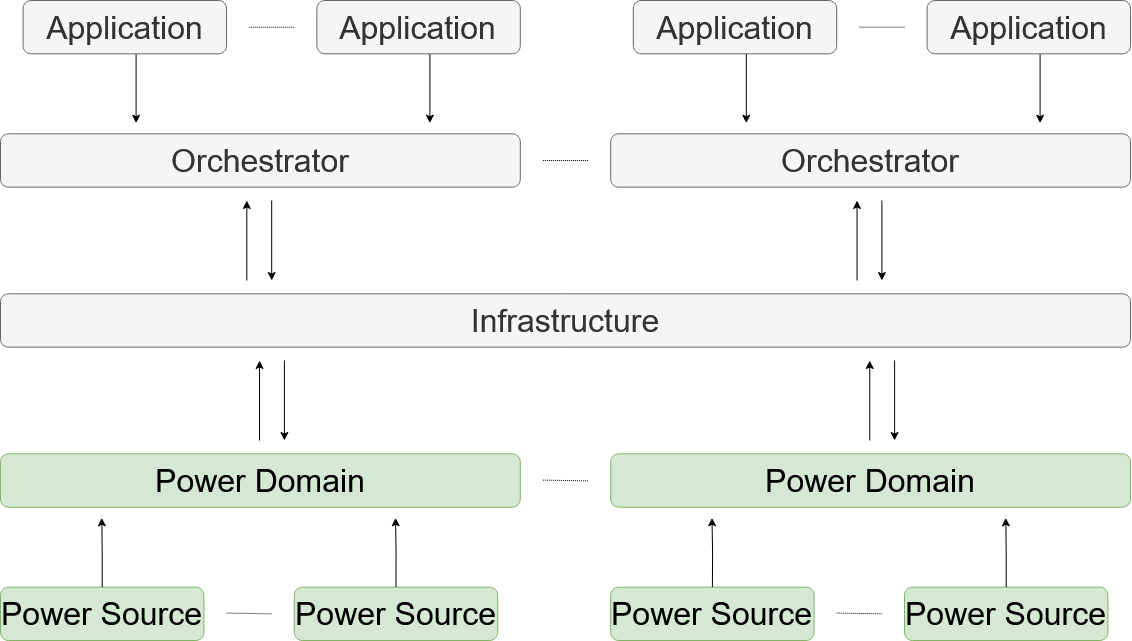
\includegraphics[width=0.8\textwidth]{images/Architecture.pdf}
    ~
    \caption{Architecture overview showing interactions between layers.}
    \label{fig:archtecture}
\end{figure}


In general, Extended LEAF was designed in an manner that would compliment the existing simulation framework but not have a mandated requirement for its features to be incorporated to carry out simulations.
As such, the extension was designed to be loosely coupled to the existing framework \citep{looseCoupling}, therefore allowing for existing simulations and scenarios to be performed under no restrictions to realise any power source or power domain.
The framework achieves this by allowing the power layer to have an unrestricted view of the underlying infrastructure of the model, being able to query the state of entities in the above layer and having the power domain carry out necessary actions on the infrastructure.
In particular, the framework operates within a unified discrete event space allowing for a power domain to run simultaneously, as such we can realise interactions between power sources and infrastructure through keeping associations between the two layers respectively.

Despite entities within the infrastructure having the optional ability to indicate a positional location, power sources do not consider share this property and assumes that a power is able to be supplied
As a result of this, Extended LEAF expects power sources to be defined by the user in the unit of watts.


As previously mentioned, power sources interact with the infrastructure through the power domain and can receive entities through the distribution mechanism employed by it.
The remaining part of this section will proceed to describe why

\subsection{Static Power Sources}\label{subsec:static-power-sources}
When a power source is defined as static, the user must provide the entities from the infrastructure that they want to associate the source to.
From this, the power source will only distribute power to these provided entities and disregard the distribution process of the power domain, if a situation occurs where the power source can no longer provide power to these entities then all nodes and links associated will be powered off and any tasks running will be paused until power can be provided to the entity.
The model provides this ability to allow for scenarios when a simulation requires various power sources but needs to impose restrictions on particular entities in the infrastructure.

\subsection{Dynamic Power Sources}\label{subsec:dynamic-power-sources}
When a power source is defined as dynamic, the user will associate any entities within the infrastructure to the power domain, represented as $\mathbf{I_{pd} \in I}$, where $\mathbf{I}$ encompasses all nodes and links denoted as $\mathbf{\{N\} \cup \{L\}}$.
From this the responsibility to allocate a power source resolves to the power domains distribution method discussed in \ref{subsec:distributing-entities}, whether being the default algorithm provided by Extended LEAF or one defined by the user.
Unlike the statically defined power source configuration, when a scenario occurs where an infrastructure entity is not allocated directly to a power source the simulation fails.\\

\subsection{Power Source Types}\label{subsec:power-source-types}
In order to realise the ability to fluctuate power availability and carbon intensity, Extended LEAF introduces Power Types for power sources.
Power sources should be characterised into groups based on attributes inherent to them.
For instance, an assumption made by Extended LEAF is the idea that real life power sources such as the National Energy Grid in the UK
3 main types:
renewable:
    - static carbon intensity
    - variable power
mixed
    - variable carbon intensity (as a result of combo of non)
    - assumed unlimited power
battery
    - small static carbon intensity
    - finite power
    - power is provided from another source and is recharged by them, providing source emits the carbon obvisouly

\subsection{Historical Data}\label{subsec:data Reading}
To realise the requirement of a fluctuating power availability, Extended LEAF models a power source's power availability and carbon intensity on historical and approximate data.
 - As this is an estimation can rely on historical data to represent trends in both power and carbon intensity
    - type is based on power source type
    - user is able to decide what data is used and can pass their own in


What did you do to implement this idea, and what technical achievements did you make?
\section{Guidance}
You can't talk about everything. Cover the high level first, then cover important, relevant or impressive details.



\section{General points}

These points apply to the whole dissertation, not just this chapter.



\subsection{Figures}
\emph{Always} refer to figures included, like Figure \ref{fig:relu}, in the body of the text. Include full, explanatory captions and make sure the figures look good on the page.
You may include multiple figures in one float, as in Figure \ref{fig:synthetic}, using \texttt{subcaption}, which is enabled in the template.



% Figures are important. Use them well.
\begin{figure}
    \centering
    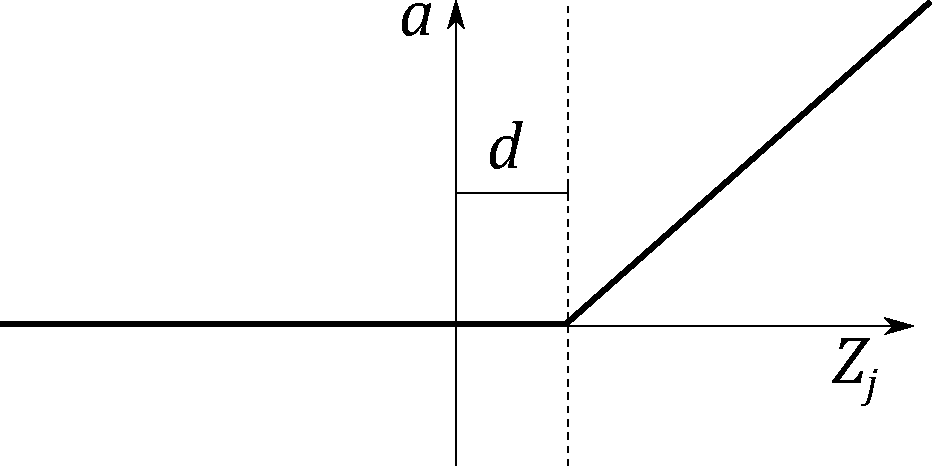
\includegraphics[width=0.5\linewidth]{images/relu.pdf}    

    \caption{In figure captions, explain what the reader is looking at: ``A schematic of the rectifying linear unit, where $a$ is the output amplitude,
    $d$ is a configurable dead-zone, and $Z_j$ is the input signal'', as well as why the reader is looking at this: 
    ``It is notable that there is no activation \emph{at all} below 0, which explains our initial results.'' 
    \textbf{Use vector image formats (.pdf) where possible}. Size figures appropriately, and do not make them over-large or too small to read.
    }

    % use the notation fig:name to cross reference a figure
    \label{fig:relu} 
\end{figure}


\begin{figure}
    \centering
    \begin{subfigure}[b]{0.45\textwidth}
        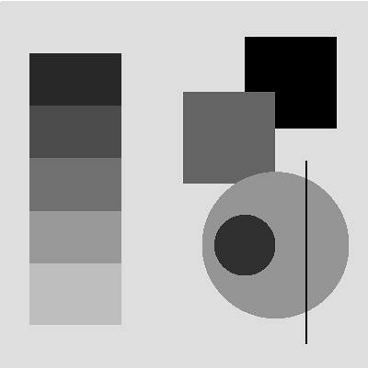
\includegraphics[width=\textwidth]{images/synthetic.png}
        \caption{Synthetic image, black on white.}
        \label{fig:syn1}
    \end{subfigure}
    ~ %add desired spacing between images, e. g. ~, \quad, \qquad, \hfill etc. 
      %(or a blank line to force the subfigure onto a new line)
    \begin{subfigure}[b]{0.45\textwidth}
        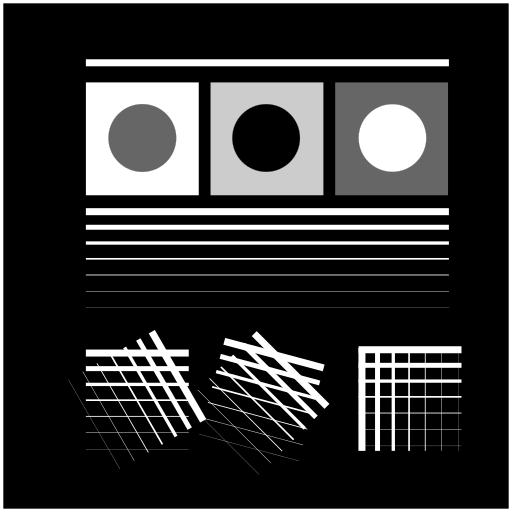
\includegraphics[width=\textwidth]{images/synthetic_2.png}
        \caption{Synthetic image, white on black.}
        \label{fig:syn2}
    \end{subfigure}
    ~ %add desired spacing between images, e. g. ~, \quad, \qquad, \hfill etc. 
    %(or a blank line to force the subfigure onto a new line)    
    \caption{Synthetic test images for edge detection algorithms. \subref{fig:syn1} shows various gray levels that require an adaptive algorithm. \subref{fig:syn2}
    shows more challenging edge detection tests that have crossing lines. Fusing these into full segments typically requires algorithms like the Hough transform.
    This is an example of using subfigures, with \texttt{subref}s in the caption.
    }\label{fig:synthetic}
\end{figure}

\clearpage

\subsection{Equations}

Equations should be typeset correctly and precisely. Make sure you get parenthesis sizing correct, and punctuate equations correctly 
(the comma is important and goes \textit{inside} the equation block). Explain any symbols used clearly if not defined earlier. 

For example, we might define:
\begin{equation}
    \hat{f}(\xi) = \frac{1}{2}\left[ \int_{-\infty}^{\infty} f(x) e^{2\pi i x \xi} \right],
\end{equation}    
where $\hat{f}(\xi)$ is the Fourier transform of the time domain signal $f(x)$.

\subsection{Algorithms}
Algorithms can be set using \texttt{algorithm2e}, as in Algorithm \ref{alg:metropolis}.

% NOTE: line ends are denoted by \; in algorithm2e
\begin{algorithm}
    \DontPrintSemicolon
    \KwData{$f_X(x)$, a probability density function returing the density at $x$.\; $\sigma$ a standard deviation specifying the spread of the proposal distribution.\;
    $x_0$, an initial starting condition.}
    \KwResult{$s=[x_1, x_2, \dots, x_n]$, $n$ samples approximately drawn from a distribution with PDF $f_X(x)$.}
    \Begin{
        $s \longleftarrow []$\;
        $p \longleftarrow f_X(x)$\;
        $i \longleftarrow 0$\;
        \While{$i < n$}
        {
            $x^\prime \longleftarrow \mathcal{N}(x, \sigma^2)$\;
            $p^\prime \longleftarrow f_X(x^\prime)$\;
            $a \longleftarrow \frac{p^\prime}{p}$\;
            $r \longleftarrow U(0,1)$\;
            \If{$r<a$}
            {
                $x \longleftarrow x^\prime$\;
                $p \longleftarrow f_X(x)$\;
                $i \longleftarrow i+1$\;
                append $x$ to $s$\;
            }
        }
    }
    
\caption{The Metropolis-Hastings MCMC algorithm for drawing samples from arbitrary probability distributions, 
specialised for normal proposal distributions $q(x^\prime|x) = \mathcal{N}(x, \sigma^2)$. The symmetry of the normal distribution means the acceptance rule takes the simplified form.}\label{alg:metropolis}
\end{algorithm}

\subsection{Tables}

If you need to include tables, like Table \ref{tab:operators}, use a tool like https://www.tablesgenerator.com/ to generate the table as it is
extremely tedious otherwise. 

\begin{table}[]
    \caption{The standard table of operators in Python, along with their functional equivalents from the \texttt{operator} package. Note that table
    captions go above the table, not below. Do not add additional rules/lines to tables. }\label{tab:operators}
    %\tt 
    \rowcolors{2}{}{gray!3}
    \begin{tabular}{@{}lll@{}}
    %\toprule
    \textbf{Operation}    & \textbf{Syntax}                & \textbf{Function}                            \\ %\midrule % optional rule for header
    Addition              & \texttt{a + b}                          & \texttt{add(a, b)}                                    \\
    Concatenation         & \texttt{seq1 + seq2}                    & \texttt{concat(seq1, seq2)}                           \\
    Containment Test      & \texttt{obj in seq}                     & \texttt{contains(seq, obj)}                           \\
    Division              & \texttt{a / b}                          & \texttt{div(a, b) }  \\
    Division              & \texttt{a / b}                          & \texttt{truediv(a, b) } \\
    Division              & \texttt{a // b}                         & \texttt{floordiv(a, b)}                               \\
    Bitwise And           & \texttt{a \& b}                         & \texttt{and\_(a, b)}                                  \\
    Bitwise Exclusive Or  & \texttt{a \textasciicircum b}           & \texttt{xor(a, b)}                                    \\
    Bitwise Inversion     & \texttt{$\sim$a}                        & \texttt{invert(a)}                                    \\
    Bitwise Or            & \texttt{a | b}                          & \texttt{or\_(a, b)}                                   \\
    Exponentiation        & \texttt{a ** b}                         & \texttt{pow(a, b)}                                    \\
    Identity              & \texttt{a is b}                         & \texttt{is\_(a, b)}                                   \\
    Identity              & \texttt{a is not b}                     & \texttt{is\_not(a, b)}                                \\
    Indexed Assignment    & \texttt{obj{[}k{]} = v}                 & \texttt{setitem(obj, k, v)}                           \\
    Indexed Deletion      & \texttt{del obj{[}k{]}}                 & \texttt{delitem(obj, k)}                              \\
    Indexing              & \texttt{obj{[}k{]}}                     & \texttt{getitem(obj, k)}                              \\
    Left Shift            & \texttt{a \textless{}\textless b}       & \texttt{lshift(a, b)}                                 \\
    Modulo                & \texttt{a \% b}                         & \texttt{mod(a, b)}                                    \\
    Multiplication        & \texttt{a * b}                          & \texttt{mul(a, b)}                                    \\
    Negation (Arithmetic) & \texttt{- a}                            & \texttt{neg(a)}                                       \\
    Negation (Logical)    & \texttt{not a}                          & \texttt{not\_(a)}                                     \\
    Positive              & \texttt{+ a}                            & \texttt{pos(a)}                                       \\
    Right Shift           & \texttt{a \textgreater{}\textgreater b} & \texttt{rshift(a, b)}                                 \\
    Sequence Repetition   & \texttt{seq * i}                        & \texttt{repeat(seq, i)}                               \\
    Slice Assignment      & \texttt{seq{[}i:j{]} = values}          & \texttt{setitem(seq, slice(i, j), values)}            \\
    Slice Deletion        & \texttt{del seq{[}i:j{]}}               & \texttt{delitem(seq, slice(i, j))}                    \\
    Slicing               & \texttt{seq{[}i:j{]}}                   & \texttt{getitem(seq, slice(i, j))}                    \\
    String Formatting     & \texttt{s \% obj}                       & \texttt{mod(s, obj)}                                  \\
    Subtraction           & \texttt{a - b}                          & \texttt{sub(a, b)}                                    \\
    Truth Test            & \texttt{obj}                            & \texttt{truth(obj)}                                   \\
    Ordering              & \texttt{a \textless b}                  & \texttt{lt(a, b)}                                     \\
    Ordering              & \texttt{a \textless{}= b}               & \texttt{le(a, b)}                                     \\
    % \bottomrule
    \end{tabular}
    \end{table}
\subsection{Code}

Avoid putting large blocks of code in the report (more than a page in one block, for example). Use syntax highlighting if possible, as in Listing \ref{lst:callahan}.

\begin{lstlisting}[language=python, float, caption={The algorithm for packing the $3\times 3$ outer-totalistic binary CA successor rule into a 
    $16\times 16\times 16\times 16$ 4 bit lookup table, running an equivalent, notionally 16-state $2\times 2$ CA.}, label=lst:callahan]
    def create_callahan_table(rule="b3s23"):
        """Generate the lookup table for the cells."""        
        s_table = np.zeros((16, 16, 16, 16), dtype=np.uint8)
        birth, survive = parse_rule(rule)

        # generate all 16 bit strings
        for iv in range(65536):
            bv = [(iv >> z) & 1 for z in range(16)]
            a, b, c, d, e, f, g, h, i, j, k, l, m, n, o, p = bv

            # compute next state of the inner 2x2
            nw = apply_rule(f, a, b, c, e, g, i, j, k)
            ne = apply_rule(g, b, c, d, f, h, j, k, l)
            sw = apply_rule(j, e, f, g, i, k, m, n, o)
            se = apply_rule(k, f, g, h, j, l, n, o, p)

            # compute the index of this 4x4
            nw_code = a | (b << 1) | (e << 2) | (f << 3)
            ne_code = c | (d << 1) | (g << 2) | (h << 3)
            sw_code = i | (j << 1) | (m << 2) | (n << 3)
            se_code = k | (l << 1) | (o << 2) | (p << 3)

            # compute the state for the 2x2
            next_code = nw | (ne << 1) | (sw << 2) | (se << 3)

            # get the 4x4 index, and write into the table
            s_table[nw_code, ne_code, sw_code, se_code] = next_code

        return s_table

\end{lstlisting}

%==================================================================================================================================
\chapter{Evaluation} \label{chp:evaluation}
How good is your solution? How well did you solve the general problem, and what evidence do you have to support that?

When the user sets out to carry out a simulation, the user should reference Figure \ref{fig:archtecture} and work from the bottom up
\section{Introduction}\label{sec:eval-intro}
\section{Introduction}\label{sec:eval-example1}
\section{Introduction}\label{sec:eval-example2}
\section{Introduction}\label{sec:eval-example3}
\section{Introduction}\label{sec:eval-example4}
\section{Introduction}\label{sec:eval-example5}
\section{Introduction}\label{sec:eval-example6}
\section{Introduction}\label{sec:eval-example7}

\section{Guidance}
\begin{itemize}
    \item
        Ask specific questions that address the general problem.
    \item
        Answer them with precise evidence (graphs, numbers, statistical
        analysis, qualitative analysis).
    \item
        Be fair and be scientific.
    \item
        The key thing is to show that you know how to evaluate your work, not
        that your work is the most amazing product ever.
\end{itemize}

\section{Evidence}
Make sure you present your evidence well. Use appropriate visualisations, reporting techniques and statistical analysis, as appropriate.

If you visualise, follow the basic rules, as illustrated in Figure \ref{fig:boxplot}:
\begin{itemize}
\item Label everything correctly (axis, title, units).
\item Caption thoroughly.
\item Reference in text.
\item \textbf{Include appropriate display of uncertainty (e.g. error bars, Box plot)}
\item Minimize clutter.
\end{itemize}

See the file \texttt{guide\_to\_visualising.pdf} for further information and guidance.

\begin{figure}
    \centering
    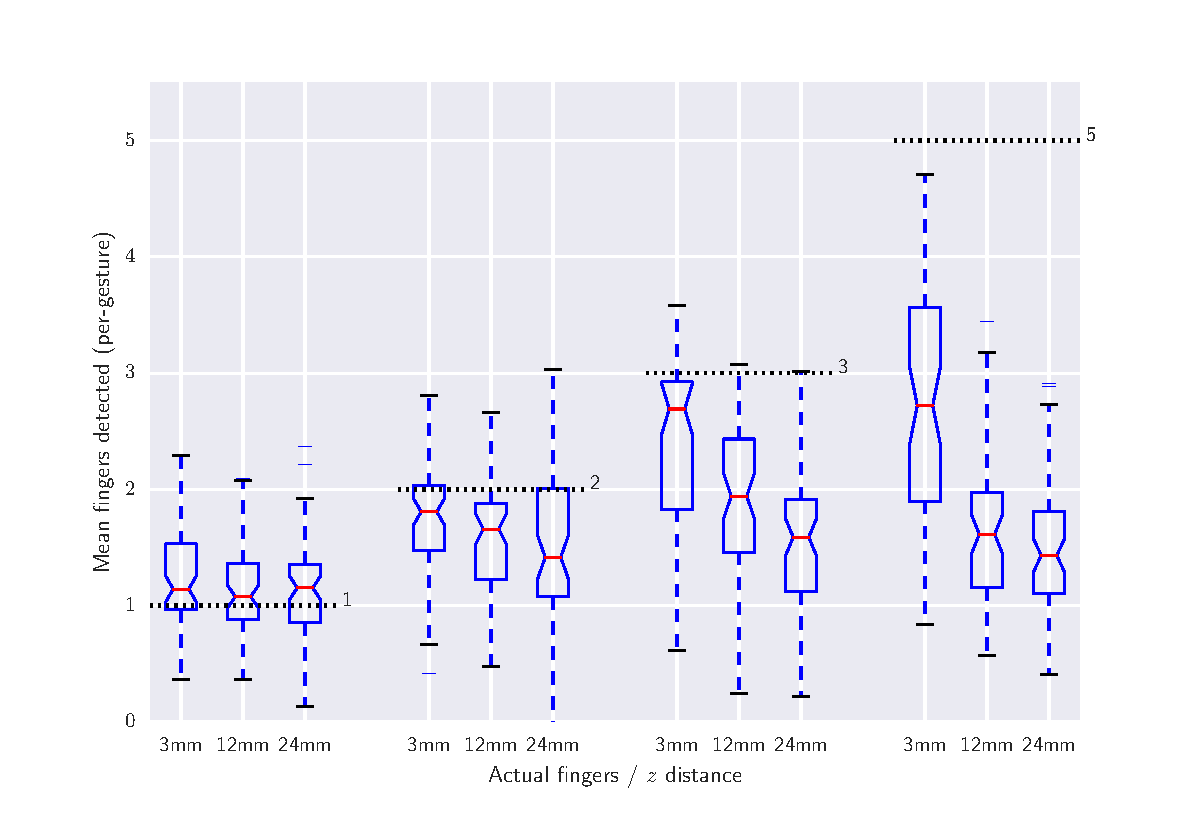
\includegraphics[width=1.0\linewidth]{images/boxplot_finger_distance.pdf}    

    \caption{Average number of fingers detected by the touch sensor at different heights above the surface, averaged over all gestures. Dashed lines indicate
    the true number of fingers present. The Box plots include bootstrapped uncertainty notches for the median. It is clear that the device is biased toward 
    undercounting fingers, particularly at higher $z$ distances.
    }

    % use the notation fig:name to cross reference a figure
    \label{fig:boxplot} 
\end{figure}


%==================================================================================================================================
\chapter{Conclusion}    
Summarise the whole project for a lazy reader who didn't read the rest (e.g. a prize-awarding committee).
\section{Guidance}
\begin{itemize}
    \item
        Summarise briefly and fairly.
    \item
        You should be addressing the general problem you introduced in the
        Introduction.        
    \item
        Include summary of concrete results (``the new compiler ran 2x
        faster'')
    \item
        Indicate what future work could be done, but remember: \textbf{you
        won't get credit for things you haven't done}.
\end{itemize}
- mention future intrest and collaborations with other students
- mention to incorperate an automatic priorising system to allow for dynamic carbon intensity sources like Grid to have their priority change
%==================================================================================================================================
%
% 
%==================================================================================================================================
%  APPENDICES  

\begin{appendices}

\chapter{Appendices}

Typical inclusions in the appendices are:

\begin{itemize}
\item
  Copies of ethics approvals (required if obtained)
\item
  Copies of questionnaires etc. used to gather data from subjects.
\item
  Extensive tables or figures that are too bulky to fit in the main body of
  the report, particularly ones that are repetitive and summarised in the body.

\item Outline of the source code (e.g. directory structure), or other architecture documentation like class diagrams.

\item User manuals, and any guides to starting/running the software.

\end{itemize}

\textbf{Don't include your source code in the appendices}. It will be
submitted separately.

\end{appendices}

%==================================================================================================================================
%   BIBLIOGRAPHY   

% The bibliography style is abbrvnat
% The bibliography always appears last, after the appendices.

\bibliographystyle{abbrvnat}

\bibliography{l4proj}

\end{document}
